\section{server}
Package base per le funzionalità del server.\begin{center}
		\begin{figure}[H]
			\centering 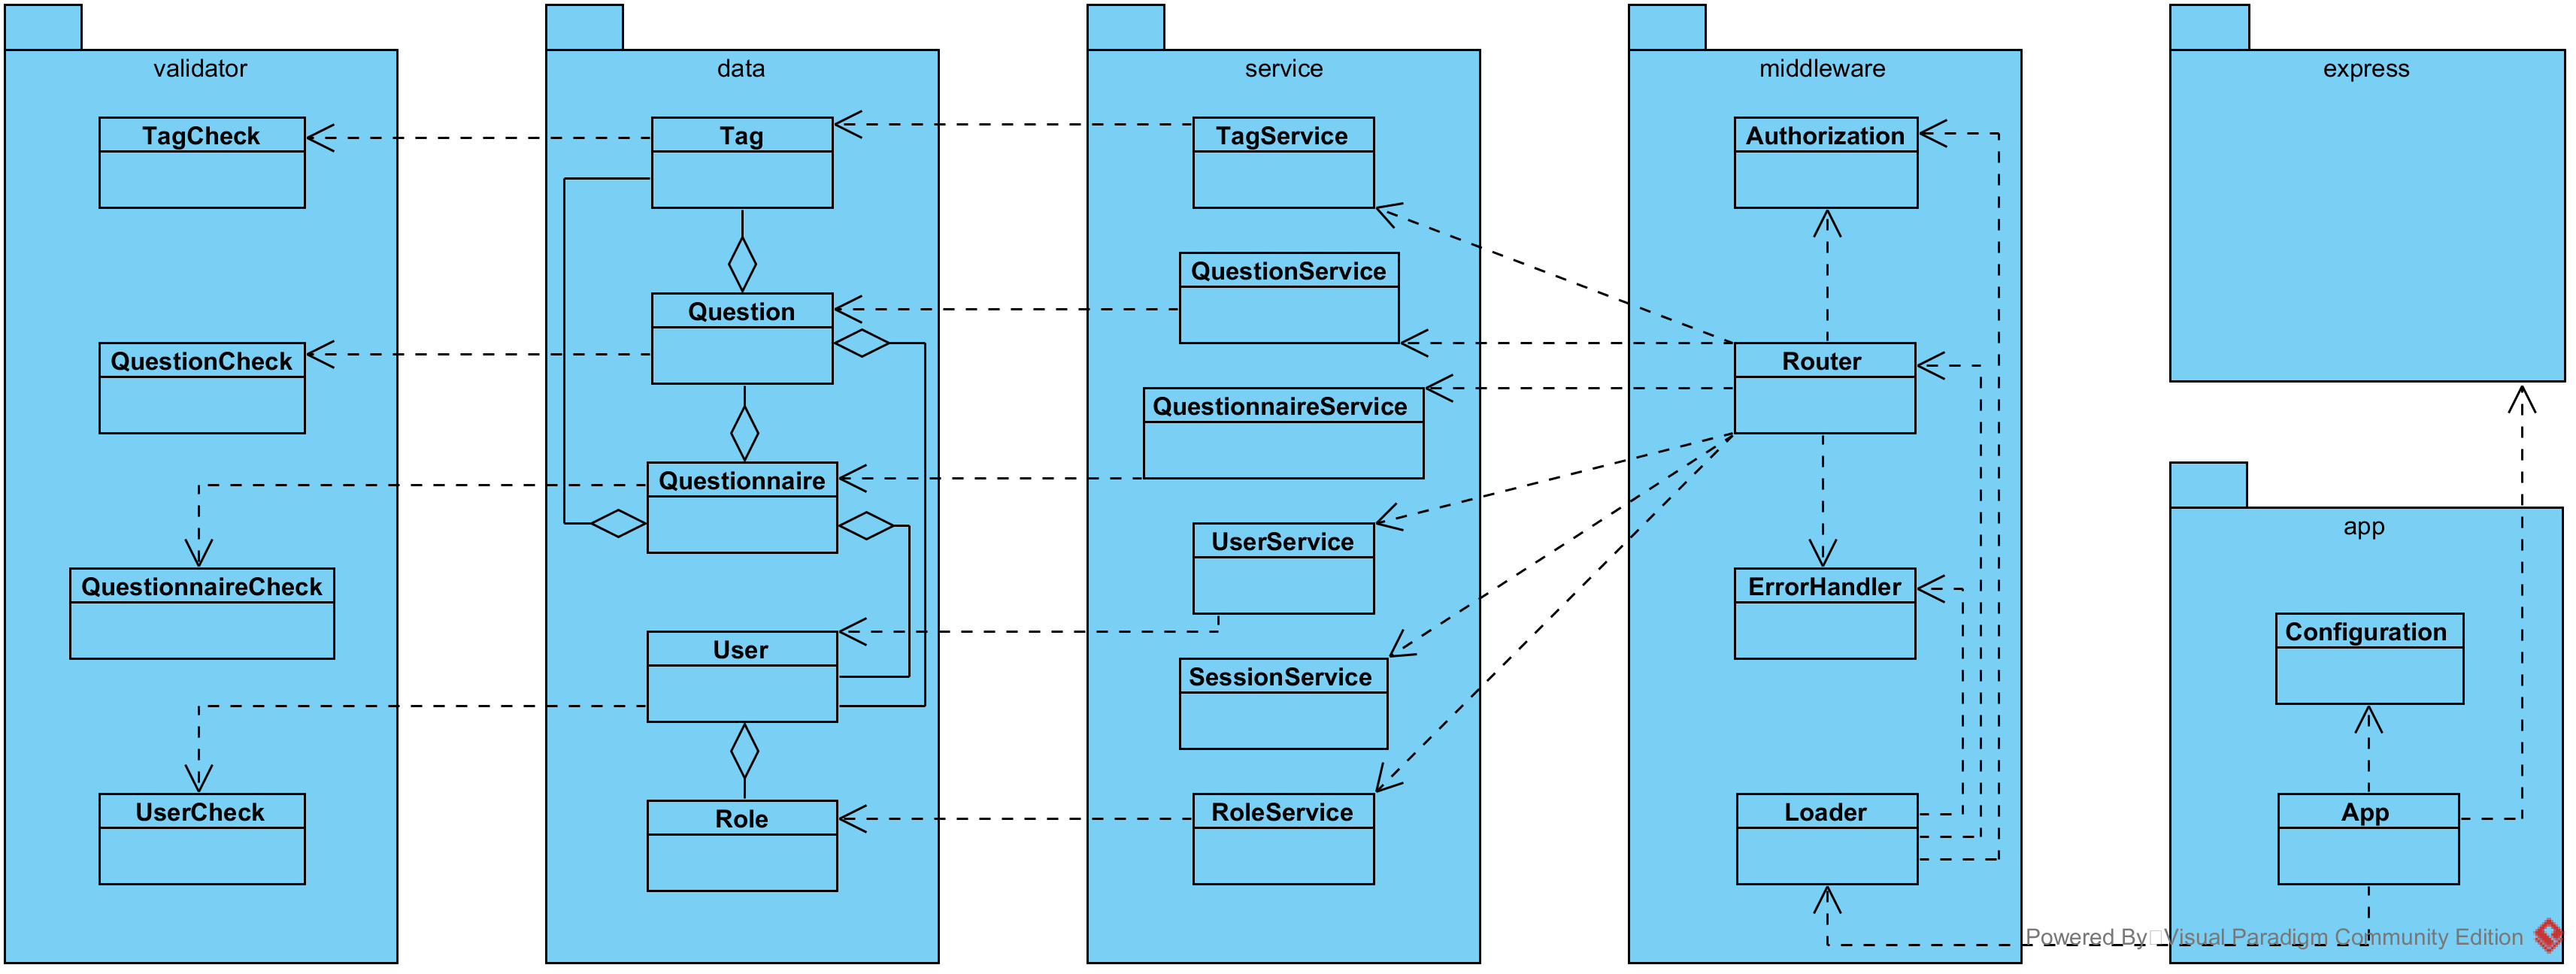
\includegraphics[scale=4, max width=\textwidth, max height=\myheight]{../img/diagrammiClassi/server.png}
			\caption{Diagramma package - server}
		\end{figure}
	\end{center}\subsection{server::app}
Questo Package ha il compito di fornire la configurazione e avviare il web server di Quizzipedia.\begin{center}
		\begin{figure}[H]
			\centering 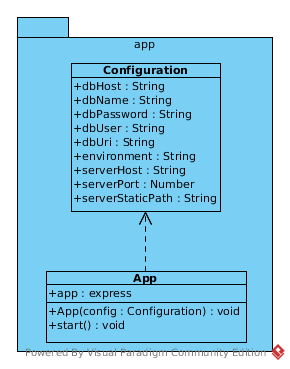
\includegraphics[scale=4, max width=\textwidth, max height=\myheight]{../img/diagrammiClassi/server/app.png}
			\caption{Diagramma package - server::app}
		\end{figure}
	\end{center}\hypertarget{server::app::App}{}
\subsubsection[App]{server::app::App}
\begin{center}
			\begin{figure}[H]
				\centering 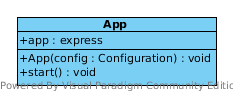
\includegraphics[scale=4, max width=\textwidth, max height=\myheight]{../img/diagrammiClassi/server/app/App.png}
				\caption{Diagramma classe - server::app::App}
			\end{figure}
		\end{center}\begin{description}
\item[Descrizione] \hfill \\
 Classe che si occupa di avviare il server e di invocare i middleware
\item[Utilizzo] \hfill \\
 Viene utilizzata per avviare il server dell'applicazione
\item[Attributi] \hfill \\
 \vspace{-7mm}
\begin{itemize}
\item app : Express (Oggetto che rappresenta l'applicazione Express)
\end{itemize}

\item[Metodi] \hfill \\
 \vspace{-7mm}
\begin{itemize}
\item App(config : Configuration) (Costruttore della classe)\begin{itemize}
\item config (Configurazione per l'inizializzazione dell'applicazione)
\end{itemize}

\item start() : void (Metodo che avvia il server. Non ritorna il controllo fino a che il server è in funzione)
\end{itemize}

\end{description}

\vspace{0.5cm}
\hypertarget{server::app::Configuration}{}
\subsubsection[Configuration]{server::app::Configuration}
\begin{center}
			\begin{figure}[H]
				\centering 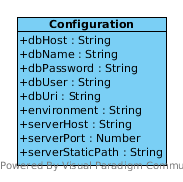
\includegraphics[scale=4, max width=\textwidth, max height=\myheight]{../img/diagrammiClassi/server/app/Configuration.png}
				\caption{Diagramma classe - server::app::Configuration}
			\end{figure}
		\end{center}\begin{description}
\item[Descrizione] \hfill \\
 Classe che rappresenta i parametri di configurazione del server
\item[Utilizzo] \hfill \\
 Viene utilizzata per definire le configurazioni dell'applicazione, passando un oggetto di questa classe al costruttore della classe App
\item[Attributi] \hfill \\
 \vspace{-7mm}
\begin{itemize}
\item environment : String (Variabile d'ambiente che informa se l'applicazione deve essere eseguita in modalità development o production)
\item serverHost : String (Indirizzo IP dell'host)
\item serverPort : Number (Porta su cui il server deve mettersi in ascolto)
\item serverStaticPath : String (Percorso della cartella che il server utilizza per fornire file statici)
\item dbHost : String (Stringa che identifica l'host del database)
\item dbName : String (Nome del database dell'applicazione)
\item dbUser : String (Username per connettersi al database)
\item dbPassword : String (Password per connettersi al database)
\item dbUri : String (Stringa di connessione al database)
\end{itemize}

\end{description}

\vspace{0.5cm}
\subsection{server::express}
Express è un framework minimale, basato sul design pattern architetturale MVC per creare applicazioni web con Node.js. Express offre funzionalità che semplificano e aumentano le potenzialità di Node.js, fornendo una migliore implementazione del sistema di routing, incrementando
le funzioni di richiesta e risposta estendendole per una maggior flessibilità, integrando nuovi middleware, ed agevolando la realizzazione delle viste.
Express non limita l’utente nella scelta del linguaggio di templating, lo aiuta a gestire le route, le request e le view.
\subsection{server::middleware}
Package che si occupa di ricevere richieste, richiamare il servizio adatto e restituire le risposte.\begin{center}
		\begin{figure}[H]
			\centering 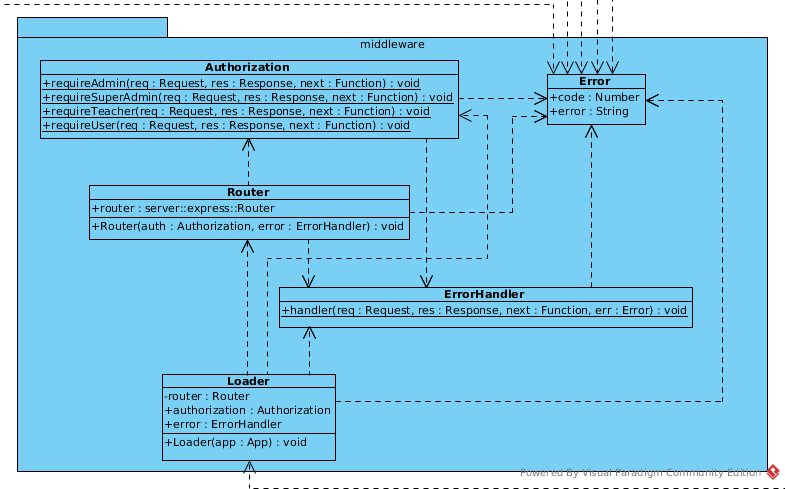
\includegraphics[scale=4, max width=\textwidth, max height=\myheight]{../img/diagrammiClassi/server/middleware.png}
			\caption{Diagramma package - server::middleware}
		\end{figure}
	\end{center}\hypertarget{server::middleware::Router}{}
\subsubsection[Router]{server::middleware::Router}
\begin{center}
			\begin{figure}[H]
				\centering 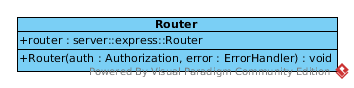
\includegraphics[scale=4, max width=\textwidth, max height=\myheight]{../img/diagrammiClassi/server/middleware/Router.png}
				\caption{Diagramma classe - server::middleware::Router}
			\end{figure}
		\end{center}\begin{description}
\item[Descrizione] \hfill \\
 Classe che si occupa della richiesta di risorse
\item[Utilizzo] \hfill \\
 Si occupa di smistare la richiesta in base all’URI ricevuto e ad invocare l’opportuno servizio
\item[Attributi] \hfill \\
 \vspace{-7mm}
\begin{itemize}
\item router : express.Router (Oggetto Router di Express)
\end{itemize}

\item[Metodi] \hfill \\
 \vspace{-7mm}
\begin{itemize}
\item Router(auth : Authorization, error : ErrorHandler) (Costruttore che definisce per ogni richiesta il corrispondente controller che dovrà gestirla verificando i permessi del richiedente)\begin{itemize}
\item auth (Istanza dell'oggetto Authorization)
\item error (Istanza del gestore degli errori)
\end{itemize}

\end{itemize}

\end{description}

\vspace{0.5cm}
\hypertarget{server::middleware::Authorization}{}
\subsubsection[Authorization]{server::middleware::Authorization}
\begin{center}
			\begin{figure}[H]
				\centering 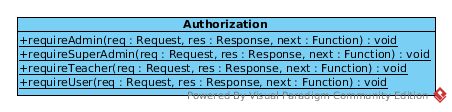
\includegraphics[scale=4, max width=\textwidth, max height=\myheight]{../img/diagrammiClassi/server/middleware/Authorization.png}
				\caption{Diagramma classe - server::middleware::Authorization}
			\end{figure}
		\end{center}\begin{description}
\item[Descrizione] \hfill \\
 Classe che si occupa dell’autorizzazione delle richieste
\item[Utilizzo] \hfill \\
 Viene utilizzata per verificare i permessi dell'utente per ogni richiesta
\item[Metodi] \hfill \\
 \vspace{-7mm}
\begin{itemize}
\item requireUser(req : Request, res : Response, next : Function) : void (Metodo che verifica che l’utente autenticato richiamando il successivo middleware in caso affermativo, rispondendo con un errore altrimenti)\begin{itemize}
\item req (Questo oggetto rappresenta la richiesta arrivata al server che il metodo deve gestire)
\item res (Questo oggetto rappresenta la risposta che il server dovrà inviare al termine dell'elaborazione)
\item next (Questo parametro rappresenta la callback che il metodo dovrà chiamare al termine dell’elaborazione)
\end{itemize}

\item requireTeacher(req : Request, res : Response, next : Function) : void (Metodo che verifica che l’utente autenticato sia almeno di tipo docente richiamando il successivo middleware in caso affermativo, rispondendo con un errore altrimenti)\begin{itemize}
\item req (Questo oggetto rappresenta la richiesta arrivata al server che il metodo deve gestire)
\item res (Questo oggetto rappresenta la risposta che il server dovrà inviare al termine dell'elaborazione)
\item next (Questo parametro rappresenta la callback che il metodo dovrà chiamare al termine dell’elaborazione)
\end{itemize}

\item requireAdmin(req : Request, res : Response, next : Function) : void (Metodo che verifica che l’utente autenticato sia almeno di tipo amministratore richiamando il successivo middleware in caso affermativo, rispondendo con un errore altrimenti)\begin{itemize}
\item req (Questo oggetto rappresenta la richiesta arrivata al server che il metodo deve gestire)
\item res (Questo oggetto rappresenta la risposta che il server dovrà inviare al termine dell'elaborazione)
\item next (Questo parametro rappresenta la callback che il metodo dovrà chiamare al termine dell’elaborazione)
\end{itemize}

\item requireSuperAdmin(req : Request, res : Response, next : Function) : void (Metodo che verifica che l’utente autenticato sia almeno di tipo proprietario richiamando il successivo middleware in caso affermativo, rispondendo con un errore altrimenti)\begin{itemize}
\item req (Questo oggetto rappresenta la richiesta arrivata al server che il metodo deve gestire)
\item res (Questo oggetto rappresenta la risposta che il server dovrà inviare al termine dell'elaborazione)
\item next (Questo parametro rappresenta la callback che il metodo dovrà chiamare al termine dell’elaborazione)
\end{itemize}

\end{itemize}

\end{description}

\vspace{0.5cm}
\hypertarget{server::middleware::Loader}{}
\subsubsection[Loader]{server::middleware::Loader}
\begin{center}
			\begin{figure}[H]
				\centering 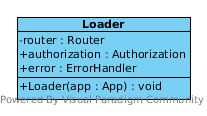
\includegraphics[scale=4, max width=\textwidth, max height=\myheight]{../img/diagrammiClassi/server/middleware/Loader.png}
				\caption{Diagramma classe - server::middleware::Loader}
			\end{figure}
		\end{center}\begin{description}
\item[Descrizione] \hfill \\
 Classe utilizzata per istanziare tutti i middleware per l'applicazione
\item[Utilizzo] \hfill \\
 Viene utilizzato per istanziare in modo nascosto all’applicazione tutti i middleware presenti nel componente server::middleware
\item[Attributi] \hfill \\
 \vspace{-7mm}
\begin{itemize}
\item authorization : Authorization (Middleware che si occupa dell'autorizzazione delle richieste)
\item error : ErrorHandler (Middleware che gestire la visualizzazione degli errori)
\item router : Router (Middleware per gestire il reindirizzamento delle richieste)
\end{itemize}

\item[Metodi] \hfill \\
 \vspace{-7mm}
\begin{itemize}
\item Loader(app : App) (Costruttore che inizializza tutti i middleware e imposta il router)\begin{itemize}
\item app (Applicazione su cui configurare i middleware)
\end{itemize}

\end{itemize}

\end{description}

\vspace{0.5cm}
\hypertarget{server::middleware::ErrorHandler}{}
\subsubsection[ErrorHandler]{server::middleware::ErrorHandler}
\begin{center}
			\begin{figure}[H]
				\centering 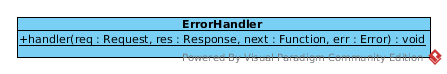
\includegraphics[scale=4, max width=\textwidth, max height=\myheight]{../img/diagrammiClassi/server/middleware/ErrorHandler.png}
				\caption{Diagramma classe - server::middleware::ErrorHandler}
			\end{figure}
		\end{center}\begin{description}
\item[Descrizione] \hfill \\
 Classe che gestisce gli errori generati nei controllers 
\item[Utilizzo] \hfill \\
 Questo middleware viene utilizzato per ultimo nella catena di gestione delle richieste di Express, in modo da gestire tutti gli errori generati precedentemente
\item[Metodi] \hfill \\
 \vspace{-7mm}
\begin{itemize}
\item handler(req : Request, res : Response, next : Function, err : Error) : void (Metodo che gestisce l'errore generato dalla richiesta)\begin{itemize}
\item req (Questo oggetto rappresenta la richiesta arrivata al server che il metodo deve gestire	)
\item res (Questo oggetto rappresenta la risposta che il server dovrà inviare al termine dell'elaborazione	)
\item next (Questo parametro rappresenta la callback che il metodo dovrà chiamare al termine dell’elaborazione	)
\item err (Questo parametro rappresenta l'oggetto  dell'errore)
\end{itemize}

\end{itemize}

\end{description}

\vspace{0.5cm}
\hypertarget{server::middleware::Error}{}
\subsubsection[Error]{server::middleware::Error}
\begin{center}
			\begin{figure}[H]
				\centering 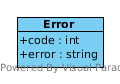
\includegraphics[scale=4, max width=\textwidth, max height=\myheight]{../img/diagrammiClassi/server/middleware/Error.png}
				\caption{Diagramma classe - server::middleware::Error}
			\end{figure}
		\end{center}\begin{description}
\item[Descrizione] \hfill \\
 Invia al client una risposta JSON con l'errore generato
\item[Utilizzo] \hfill \\
 Viene utilizzato come risposta JSON in caso di errore
\item[Attributi] \hfill \\
 \vspace{-7mm}
\begin{itemize}
\item code : Number (Identifica il codice HTTP dell'errore)
\item error : String (Messaggio dell'errore)
\end{itemize}

\end{description}

\vspace{0.5cm}
\subsection{server::data}
Package contenente le componenti che gestiscono i dati utilizzati dall'applicazione e l'interfacciamento con il database.\begin{center}
		\begin{figure}[H]
			\centering 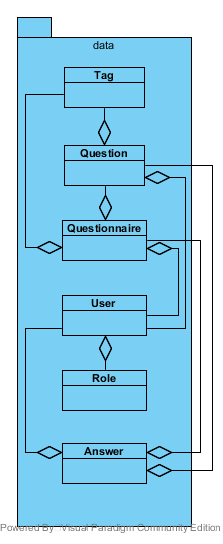
\includegraphics[scale=4, max width=\textwidth, max height=\myheight]{../img/diagrammiClassi/server/data.png}
			\caption{Diagramma package - server::data}
		\end{figure}
	\end{center}\hypertarget{server::data::Tag}{}
\subsubsection[Tag]{server::data::Tag}
\begin{center}
			\begin{figure}[H]
				\centering 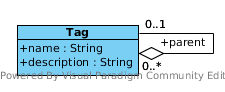
\includegraphics[scale=4, max width=\textwidth, max height=\myheight]{../img/diagrammiClassi/server/data/Tag.png}
				\caption{Diagramma classe - server::data::Tag}
			\end{figure}
		\end{center}\begin{description}
\item[Descrizione] \hfill \\
 Classe che rappresenta un argomento da assegnare alle domande o ai questionari
\item[Relazioni con altre classi] \hfill \\
 \vspace{-7mm}
\begin{description}
\item[\hyperlink{server::data::Question}{server::data::Question}] \hfill \\
 Relazione entrante, insieme di riferimenti agli argomenti associati alla domanda
\item[\hyperlink{server::data::Questionnaire}{server::data::Questionnaire}] \hfill \\
 Relazione entrante, insieme di riferimenti agli argomenti associati al questionario
\end{description}

\item[Attributi] \hfill \\
 \vspace{-7mm}
\begin{itemize}
\item name : String (Stringa identificativa dell'argomento contenente parole separate da '-')
\item parent : Tag (Riferimento all'argomento padre)
\item description : String (Breve descrizione dell'attributo)
\end{itemize}

\end{description}

\vspace{0.5cm}
\hypertarget{server::data::Questionnaire}{}
\subsubsection[Questionnaire]{server::data::Questionnaire}
\begin{center}
			\begin{figure}[H]
				\centering 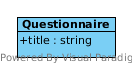
\includegraphics[scale=4, max width=\textwidth, max height=\myheight]{../img/diagrammiClassi/server/data/Questionnaire.png}
				\caption{Diagramma classe - server::data::Questionnaire}
			\end{figure}
		\end{center}\begin{description}
\item[Descrizione] \hfill \\
 Classe che rappresenta un questionario
\item[Relazioni con altre classi] \hfill \\
 \vspace{-7mm}
\begin{description}
\item[\hyperlink{server::data::Question}{server::data::Question}] \hfill \\
 Relazione uscente, insieme di riferimenti alle domande del questionario
\item[\hyperlink{server::data::Tag}{server::data::Tag}] \hfill \\
 Relazione uscente, insieme di riferimenti agli argomenti associati al questionario
\item[\hyperlink{server::data::User}{server::data::User}] \hfill \\
 Relazione uscente, riferimento all'autore del questionario
\end{description}

\item[Attributi] \hfill \\
 \vspace{-7mm}
\begin{itemize}
\item title : String (Titolo del questionario)
\item tags : Tag [] (Insieme di riferimenti agli argomenti associati al questionario)
\item author : User (Riferimento all'autore del questionario)
\item questions : Question [] (Insieme di riferimenti alle domande del questionario)
\end{itemize}

\end{description}

\vspace{0.5cm}
\hypertarget{server::data::Question}{}
\subsubsection[Question]{server::data::Question}
\begin{center}
			\begin{figure}[H]
				\centering 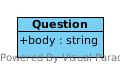
\includegraphics[scale=4, max width=\textwidth, max height=\myheight]{../img/diagrammiClassi/server/data/Question.png}
				\caption{Diagramma classe - server::data::Question}
			\end{figure}
		\end{center}\begin{description}
\item[Descrizione] \hfill \\
 Classe base comune a tutti i tipi di domanda
\item[Relazioni con altre classi] \hfill \\
 \vspace{-7mm}
\begin{description}
\item[\hyperlink{server::data::Tag}{server::data::Tag}] \hfill \\
 Relazione uscente, insieme di riferimenti agli argomenti associati alla domanda
\item[\hyperlink{server::data::User}{server::data::User}] \hfill \\
 Relazione uscente, riferimento al docente che ha creato la domanda
\item[\hyperlink{server::data::Questionnaire}{server::data::Questionnaire}] \hfill \\
 Relazione entrante, insieme di riferimenti alle domande del questionario
\end{description}

\item[Attributi] \hfill \\
 \vspace{-7mm}
\begin{itemize}
\item body : String (Stringa QML del corpo della domanda)
\item author : User (Riferimento al docente che ha creato la domanda)
\item tags : Tag [] (Insieme di riferimenti agli argomenti associati alla domanda)
\end{itemize}

\end{description}

\vspace{0.5cm}
\hypertarget{server::data::Role}{}
\subsubsection[Role]{server::data::Role}
\begin{center}
			\begin{figure}[H]
				\centering 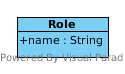
\includegraphics[scale=4, max width=\textwidth, max height=\myheight]{../img/diagrammiClassi/server/data/Role.png}
				\caption{Diagramma classe - server::data::Role}
			\end{figure}
		\end{center}\begin{description}
\item[Descrizione] \hfill \\
 Classe che rappresenta un ruolo all'interno dell'applicazione
\item[Relazioni con altre classi] \hfill \\
 \vspace{-7mm}
\begin{description}
\item[\hyperlink{server::data::User}{server::data::User}] \hfill \\
 Relazione entrante, riferimento al ruolo dell'utente nell'applicazione
\end{description}

\item[Attributi] \hfill \\
 \vspace{-7mm}
\begin{itemize}
\item name : String (Identifica la tipologia di utente)
\end{itemize}

\end{description}

\vspace{0.5cm}
\hypertarget{server::data::User}{}
\subsubsection[User]{server::data::User}
\begin{center}
			\begin{figure}[H]
				\centering 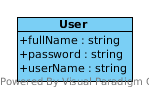
\includegraphics[scale=4, max width=\textwidth, max height=\myheight]{../img/diagrammiClassi/server/data/User.png}
				\caption{Diagramma classe - server::data::User}
			\end{figure}
		\end{center}\begin{description}
\item[Descrizione] \hfill \\
 Classe che rappresenta un utente dell'applicazione
\item[Relazioni con altre classi] \hfill \\
 \vspace{-7mm}
\begin{description}
\item[\hyperlink{server::data::Question}{server::data::Question}] \hfill \\
 Relazione entrante, riferimento al docente che ha creato la domanda
\item[\hyperlink{server::data::Questionnaire}{server::data::Questionnaire}] \hfill \\
 Relazione entrante, riferimento all'autore del questionario
\item[\hyperlink{server::data::Role}{server::data::Role}] \hfill \\
 Relazione uscente, riferimento al ruolo dell'utente nell'applicazione
\end{description}

\item[Attributi] \hfill \\
 \vspace{-7mm}
\begin{itemize}
\item fullName : String (Nome e cognome dell'utente)
\item role : Role (Riferimento al ruolo dell'utente nell'applicazione)
\item userName : String (Username univoco con la quale, in combinazione con la password, l'utente accede al sistema)
\item password : String (Hash della password utilizzata per l'accesso)
\end{itemize}

\end{description}

\vspace{0.5cm}
\subsection{server::service}
Package contenente le classi che implementano tutti i servizi offerti dall'applicazione lato server.\begin{center}
		\begin{figure}[H]
			\centering 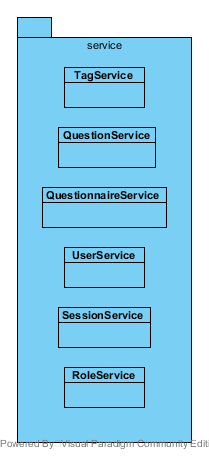
\includegraphics[scale=4, max width=\textwidth, max height=\myheight]{../img/diagrammiClassi/server/service.png}
			\caption{Diagramma package - server::service}
		\end{figure}
	\end{center}\hypertarget{server::service::UserService}{}
\subsubsection[UserService]{server::service::UserService}
\begin{center}
			\begin{figure}[H]
				\centering 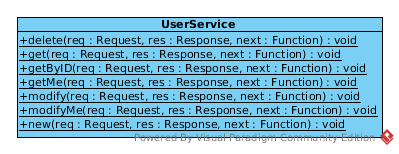
\includegraphics[scale=4, max width=\textwidth, max height=\myheight]{../img/diagrammiClassi/server/service/UserService.png}
				\caption{Diagramma classe - server::service::UserService}
			\end{figure}
		\end{center}\begin{description}
\item[Descrizione] \hfill \\
 Classe che si occupa della operazioni di inserimento, modifica e rimozione di account utenti.
\item[Utilizzo] \hfill \\
 Fornisce i dati personali degli utenti a chi ne ha il permesso di accesso ed esegue operazioni di aggiunta, modifica, rimozione e cambio di ruolo per gli utenti del sistema.
\item[Metodi] \hfill \\
 \vspace{-7mm}
\begin{itemize}
\item getByID(req : Request, res : Response, next : Function) : void (Metodo che ritorna un utente specifico)\begin{itemize}
\item req (Questo oggetto rappresenta la richiesta arrivata al server che il metodo deve gestire)
\item res (Questo oggetto rappresenta la risposta che il server dovrà inviare al termine dell'elaborazione)
\item next (Questo parametro rappresenta la callback che il metodo dovrà chiamare al termine dell’elaborazione)
\end{itemize}

\item getMe(req : Request, res : Response, next : Function) : void (Metodo che ritona l'utente loggato)\begin{itemize}
\item req (Questo oggetto rappresenta la richiesta arrivata al server che il metodo deve gestire)
\item res (Questo oggetto rappresenta la risposta che il server dovrà inviare al termine dell'elaborazione)
\item next (Questo parametro rappresenta la callback che il metodo dovrà chiamare al termine dell’elaborazione)
\end{itemize}

\item get(req : Request, res : Response, next : Function) : void (Il metodo ritorna la lista degli utenti)\begin{itemize}
\item req (Questo oggetto rappresenta la richiesta arrivata al server che il metodo deve gestire)
\item res (Questo oggetto rappresenta la risposta che il server dovrà inviare al termine dell'elaborazione)
\item next (Questo parametro rappresenta la callback che il metodo dovrà chiamare al termine dell’elaborazione)
\end{itemize}

\item new(req : Request, res : Response, next : Function) : void (Metodo che aggiunge un nuovo utente)\begin{itemize}
\item req (Questo oggetto rappresenta la richiesta arrivata al server che il metodo deve gestire)
\item res (Questo oggetto rappresenta la risposta che il server dovrà inviare al termine dell'elaborazione)
\item next (Questo parametro rappresenta la callback che il metodo dovrà chiamare al termine dell’elaborazione)
\end{itemize}

\item modify(req : Request, res : Response, next : Function) : void (Metodo che modifica i dati dell'utente specificato)\begin{itemize}
\item req (Questo oggetto rappresenta la richiesta arrivata al server che il metodo deve gestire)
\item res (Questo oggetto rappresenta la risposta che il server dovrà inviare al termine dell'elaborazione)
\item next (Questo parametro rappresenta la callback che il metodo dovrà chiamare al termine dell’elaborazione)
\end{itemize}

\item delete(req : Request, res : Response, next : Function) : void (Metodo che elimina un utente)\begin{itemize}
\item req (Questo oggetto rappresenta la richiesta arrivata al server che il metodo deve gestire)
\item res (Questo oggetto rappresenta la risposta che il server dovrà inviare al termine dell'elaborazione)
\item next (Questo parametro rappresenta la callback che il metodo dovrà chiamare al termine dell’elaborazione)
\end{itemize}

\item modifyMe(req : Request, res : Response, next : Function) : void (Modifica i dati dell'utente connesso al sistema se presente)\begin{itemize}
\item req (Questo oggetto rappresenta la richiesta arrivata al server che il metodo deve gestire)
\item res (Questo oggetto rappresenta la risposta che il server dovrà inviare al termine dell'elaborazione)
\item next (Questo parametro rappresenta la callback che il metodo dovrà chiamare al termine dell’elaborazione)
\end{itemize}

\end{itemize}

\end{description}

\vspace{0.5cm}
\hypertarget{server::service::QuestionnaireService}{}
\subsubsection[QuestionnaireService]{server::service::QuestionnaireService}
\begin{center}
			\begin{figure}[H]
				\centering 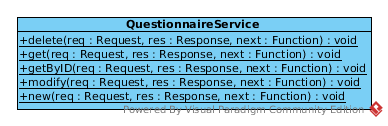
\includegraphics[scale=4, max width=\textwidth, max height=\myheight]{../img/diagrammiClassi/server/service/QuestionnaireService.png}
				\caption{Diagramma classe - server::service::QuestionnaireService}
			\end{figure}
		\end{center}\begin{description}
\item[Descrizione] \hfill \\
 Classe che si occupa di gestire questionari. È uno dei componenti product del Design Pattern Abstract Factory
\item[Utilizzo] \hfill \\
 Offre metodi per restituire questionari. Permette inoltre ad un docente di effettuare l'inserimento, la modifica, l'eliminazione di questionari
\item[Metodi] \hfill \\
 \vspace{-7mm}
\begin{itemize}
\item getByID(req : Request, res : Response, next : Function) : void (Metodo che ritorna il questionario specifico richiesto dall'utente)\begin{itemize}
\item req (Questo oggetto rappresenta la richiesta arrivata al server che il metodo deve gestire)
\item res (Questo oggetto rappresenta la risposta che il server dovrà inviare al termine dell'elaborazione)
\item next (Questo parametro rappresenta la callback che il metodo dovrà chiamare al termine dell’elaborazione)
\end{itemize}

\item get(req : Request, res : Response, next : Function) : void (Metodo che ritorna una lista di questionari)\begin{itemize}
\item req (Questo oggetto rappresenta la richiesta arrivata al server che il metodo deve gestire)
\item res (Questo oggetto rappresenta la risposta che il server dovrà inviare al termine dell'elaborazione)
\item next (Questo parametro rappresenta la callback che il metodo dovrà chiamare al termine dell’elaborazione)
\end{itemize}

\item new(req : Request, res : Response, next : Function) : void (Metodo che crea un nuovo questionario)\begin{itemize}
\item req (Questo oggetto rappresenta la richiesta arrivata al server che il metodo deve gestire)
\item res (Questo oggetto rappresenta la risposta che il server dovrà inviare al termine dell'elaborazione)
\item next (Questo parametro rappresenta la callback che il metodo dovrà chiamare al termine dell’elaborazione)
\end{itemize}

\item modify(req : Request, res : Response, next : Function) : void (Metodo che modifica un questionario specifico)\begin{itemize}
\item req (Questo oggetto rappresenta la richiesta arrivata al server che il metodo deve gestire)
\item res (Questo oggetto rappresenta la risposta che il server dovrà inviare al termine dell'elaborazione)
\item next (Questo parametro rappresenta la callback che il metodo dovrà chiamare al termine dell’elaborazione)
\end{itemize}

\item delete(req : Request, res : Response, next : Function) : void (Metodo che cancella un questionario specifico)\begin{itemize}
\item req (Questo oggetto rappresenta la richiesta arrivata al server che il metodo deve gestire)
\item res (Questo oggetto rappresenta la risposta che il server dovrà inviare al termine dell'elaborazione)
\item next (Questo parametro rappresenta la callback che il metodo dovrà chiamare al termine dell’elaborazione)
\end{itemize}

\end{itemize}

\end{description}

\vspace{0.5cm}
\hypertarget{server::service::QuestionService}{}
\subsubsection[QuestionService]{server::service::QuestionService}
\begin{center}
			\begin{figure}[H]
				\centering 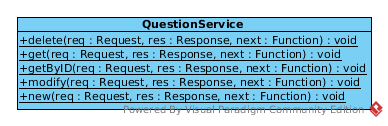
\includegraphics[scale=4, max width=\textwidth, max height=\myheight]{../img/diagrammiClassi/server/service/QuestionService.png}
				\caption{Diagramma classe - server::service::QuestionService}
			\end{figure}
		\end{center}\begin{description}
\item[Descrizione] \hfill \\
 Classe che si occupa di gestire domande. È uno dei componenti product del Design Pattern Abstract Factory
\item[Utilizzo] \hfill \\
 Offre metodi per restituire le domande. Permette inoltre ad un docente di effettuare l'inserimento, la modifica, l'eliminazione di domande
\item[Metodi] \hfill \\
 \vspace{-7mm}
\begin{itemize}
\item get(req : Request, res : Response, next : Function) : void (Metodo che ritorna una lista di domande)\begin{itemize}
\item req (Questo oggetto rappresenta la richiesta arrivata al server che il metodo deve gestire)
\item res (Questo oggetto rappresenta la risposta che il server dovrà inviare al termine dell'elaborazione)
\item next (Questo parametro rappresenta la callback che il metodo dovrà chiamare al termine dell’elaborazione)
\end{itemize}

\item getByID(req : Request, res : Response, next : Function) : void (Metodo che ritorna una domanda specifica)\begin{itemize}
\item req (Questo oggetto rappresenta la richiesta arrivata al server che il metodo deve gestire)
\item res (Questo oggetto rappresenta la risposta che il server dovrà inviare al termine dell'elaborazione)
\item next (Questo parametro rappresenta la callback che il metodo dovrà chiamare al termine dell’elaborazione)
\end{itemize}

\item new(req : Request, res : Response, next : Function) : void (Metodo che crea una nuova domanda)\begin{itemize}
\item req (Questo oggetto rappresenta la richiesta arrivata al server che il metodo deve gestire)
\item res (Questo oggetto rappresenta la risposta che il server dovrà inviare al termine dell'elaborazione)
\item next (Questo parametro rappresenta la callback che il metodo dovrà chiamare al termine dell’elaborazione)
\end{itemize}

\item modify(req : Request, res : Response, next : Function) : void (Metodo che modifica una domanda selezionata)\begin{itemize}
\item req (Questo oggetto rappresenta la richiesta arrivata al server che il metodo deve gestire)
\item res (Questo oggetto rappresenta la risposta che il server dovrà inviare al termine dell'elaborazione)
\item next (Questo parametro rappresenta la callback che il metodo dovrà chiamare al termine dell’elaborazione)
\end{itemize}

\item delete(req : Request, res : Response, next : Function) : void (Metodo che elimina una domanda selezionata)\begin{itemize}
\item req (Questo oggetto rappresenta la richiesta arrivata al server che il metodo deve gestire)
\item res (Questo oggetto rappresenta la risposta che il server dovrà inviare al termine dell'elaborazione)
\item next (Questo parametro rappresenta la callback che il metodo dovrà chiamare al termine dell’elaborazione)
\end{itemize}

\end{itemize}

\end{description}

\vspace{0.5cm}
\hypertarget{server::service::TagService}{}
\subsubsection[TagService]{server::service::TagService}
\begin{center}
			\begin{figure}[H]
				\centering 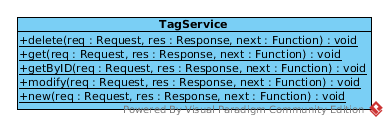
\includegraphics[scale=4, max width=\textwidth, max height=\myheight]{../img/diagrammiClassi/server/service/TagService.png}
				\caption{Diagramma classe - server::service::TagService}
			\end{figure}
		\end{center}\begin{description}
\item[Descrizione] \hfill \\
 Classe che si occupa di gestire gli argomenti. È uno dei componenti product del Design Pattern Abstract Factory
\item[Utilizzo] \hfill \\
 Offre metodi per restituire gli argomenti presenti. Permette inoltre ad un docente di effettuare l'inserimento, la modifica, l'eliminazione di argomenti
\item[Metodi] \hfill \\
 \vspace{-7mm}
\begin{itemize}
\item get(req : Request, res : Response, next : Function) : void (Metodo che ritorna la lista degli argomenti)\begin{itemize}
\item req (Questo oggetto rappresenta la richiesta arrivata al server che il metodo deve gestire)
\item res (Questo oggetto rappresenta la risposta che il server dovrà inviare al termine dell'elaborazione)
\item next (Questo parametro rappresenta la callback che il metodo dovrà chiamare al termine dell’elaborazione)
\end{itemize}

\item getByID(req : Request, res : Response, next : Function) : void (Metodo che ritorna un argomento specifico)\begin{itemize}
\item req (Questo oggetto rappresenta la richiesta arrivata al server che il metodo deve gestire)
\item res (Questo oggetto rappresenta la risposta che il server dovrà inviare al termine dell'elaborazione)
\item next (Questo parametro rappresenta la callback che il metodo dovrà chiamare al termine dell’elaborazione)
\end{itemize}

\item new(req : Request, res : Response, next : Function) : void (Metodo che crea un nuovo argomento)\begin{itemize}
\item req (Questo oggetto rappresenta la richiesta arrivata al server che il metodo deve gestire)
\item res (Questo oggetto rappresenta la risposta che il server dovrà inviare al termine dell'elaborazione)
\item next (Questo parametro rappresenta la callback che il metodo dovrà chiamare al termine dell’elaborazione)
\end{itemize}

\item modify(req : Request, res : Response, next : Function) : void (Metodo che modifica un argomento specifico)\begin{itemize}
\item req (Questo oggetto rappresenta la richiesta arrivata al server che il metodo deve gestire)
\item res (Questo oggetto rappresenta la risposta che il server dovrà inviare al termine dell'elaborazione)
\item next (Questo parametro rappresenta la callback che il metodo dovrà chiamare al termine dell’elaborazione)
\end{itemize}

\item delete(req : Request, res : Response, next : Function) : void (Metodo che elimina un argomento specifico)\begin{itemize}
\item req (Questo oggetto rappresenta la richiesta arrivata al server che il metodo deve gestire)
\item res (Questo oggetto rappresenta la risposta che il server dovrà inviare al termine dell'elaborazione)
\item next (Questo parametro rappresenta la callback che il metodo dovrà chiamare al termine dell’elaborazione)
\end{itemize}

\end{itemize}

\end{description}

\vspace{0.5cm}
\hypertarget{server::service::SessionService}{}
\subsubsection[SessionService]{server::service::SessionService}
\begin{center}
			\begin{figure}[H]
				\centering 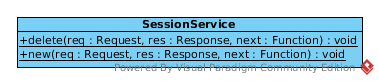
\includegraphics[scale=4, max width=\textwidth, max height=\myheight]{../img/diagrammiClassi/server/service/SessionService.png}
				\caption{Diagramma classe - server::service::SessionService}
			\end{figure}
		\end{center}\begin{description}
\item[Descrizione] \hfill \\
 Classe che si occupa della gestione della sessione dell'utente
\item[Utilizzo] \hfill \\
 Viene utilizzata per gestire il login e logout dell'utente
\item[Metodi] \hfill \\
 \vspace{-7mm}
\begin{itemize}
\item new(req : Request, res : Response, next : Function) : void (Metodo che crea una sessione con l'utente)\begin{itemize}
\item req (Questo oggetto rappresenta la richiesta arrivata al server che il metodo deve gestire)
\item res (Questo oggetto rappresenta la risposta che il server dovrà inviare al termine dell'elaborazione)
\item next (Questo parametro rappresenta la callback che il metodo dovrà chiamare al termine dell’elaborazione)
\end{itemize}

\item delete(req : Request, res : Response, next : Function) : void (Metodo che elimina la sessione dell'utente)\begin{itemize}
\item req (Questo oggetto rappresenta la richiesta arrivata al server che il metodo deve gestire)
\item res (Questo oggetto rappresenta la risposta che il server dovrà inviare al termine dell'elaborazione)
\item next (Questo parametro rappresenta la callback che il metodo dovrà chiamare al termine dell’elaborazione)
\end{itemize}

\end{itemize}

\end{description}

\vspace{0.5cm}
\hypertarget{server::service::RoleService}{}
\subsubsection[RoleService]{server::service::RoleService}
\begin{center}
			\begin{figure}[H]
				\centering 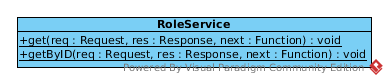
\includegraphics[scale=4, max width=\textwidth, max height=\myheight]{../img/diagrammiClassi/server/service/RoleService.png}
				\caption{Diagramma classe - server::service::RoleService}
			\end{figure}
		\end{center}\begin{description}
\item[Descrizione] \hfill \\
 Classe che rappresenta il servizio per la lettura dei ruoli utente
\item[Utilizzo] \hfill \\
 Viene utilizzata per fornire un punto d'accesso per l'elenco di tutti i ruoli dell'applicazione e la lettura di un singolo ruolo
\item[Metodi] \hfill \\
 \vspace{-7mm}
\begin{itemize}
\item get(req : Request, res : Response, next : Function) : void (Metodo che invoca il servizio per eliminare un amministratore)\begin{itemize}
\item req (Questo oggetto rappresenta la richiesta arrivata al server che il metodo deve gestire)
\item res (Questo oggetto rappresenta la risposta che il server dovrà inviare al termine dell'elaborazione)
\item next (Questo parametro rappresenta la callback che il metodo dovrà chiamare al termine dell’elaborazione)
\end{itemize}

\item getByID(req : Request, res : Response, next : Function) : void (Metodo che invoca il servizio per ottenere la lista dei ruoli o il ruolo di un utente specificato)\begin{itemize}
\item req (Questo oggetto rappresenta la richiesta arrivata al server che il metodo deve gestire)
\item res (Questo oggetto rappresenta la risposta che il server dovrà inviare al termine dell'elaborazione)
\item next (Questo parametro rappresenta la callback che il metodo dovrà chiamare al termine dell’elaborazione)
\end{itemize}

\end{itemize}

\end{description}

\vspace{0.5cm}
\subsection{server::validator}
Questo package contiene tutte le classi "validator" che hanno il compito di controllare che alcuni campi di alcuni model siano validi; esempi includo la password dell'utente, la lunghezza del nome utente o il QML di una domanda.\begin{center}
		\begin{figure}[H]
			\centering 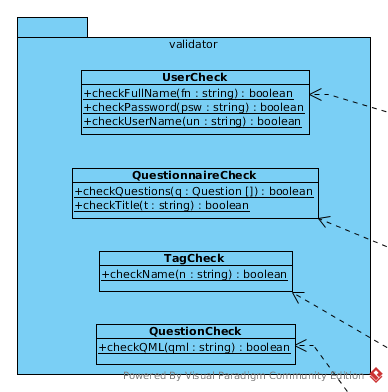
\includegraphics[scale=4, max width=\textwidth, max height=\myheight]{../img/diagrammiClassi/server/validator.png}
			\caption{Diagramma package - server::validator}
		\end{figure}
	\end{center}\hypertarget{server::validator::UserCheck}{}
\subsubsection[UserCheck]{server::validator::UserCheck}
\begin{center}
			\begin{figure}[H]
				\centering 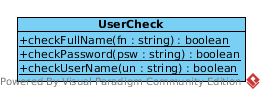
\includegraphics[scale=4, max width=\textwidth, max height=\myheight]{../img/diagrammiClassi/server/validator/UserCheck.png}
				\caption{Diagramma classe - server::validator::UserCheck}
			\end{figure}
		\end{center}\begin{description}
\item[Descrizione] \hfill \\
 Questa classe contiene tutte le funzioni di controllo della validità dei campi del model User
\item[Utilizzo] \hfill \\
 Viene utilizzata dai service per effettuare controlli sul model User
\item[Metodi] \hfill \\
 \vspace{-7mm}
\begin{itemize}
\item checkFullName(fn : String) : Boolean (Controlla che il nome completo passato contenga almeno 2 caratteri)\begin{itemize}
\item fn (Il nome completo da controllare)
\end{itemize}

\item checkPassword(psw : String) : Boolean (Controlla che la password passata contenga almeno 8 caratteri)\begin{itemize}
\item psw (La password, ovviamente in chiaro (non l'hash), da controllare)
\end{itemize}

\item checkUserName(un : String) : Boolean (Controlla che l'username passato contenga almeno 6 caratteri)\begin{itemize}
\item un (L'username da controllare)
\end{itemize}

\item checkUniqueUserName() : Boolean (Controlla se l'username passato non è presente nel sistema)
\end{itemize}

\end{description}

\vspace{0.5cm}
\hypertarget{server::validator::QuestionnaireCheck}{}
\subsubsection[QuestionnaireCheck]{server::validator::QuestionnaireCheck}
\begin{center}
			\begin{figure}[H]
				\centering 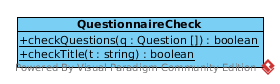
\includegraphics[scale=4, max width=\textwidth, max height=\myheight]{../img/diagrammiClassi/server/validator/QuestionnaireCheck.png}
				\caption{Diagramma classe - server::validator::QuestionnaireCheck}
			\end{figure}
		\end{center}\begin{description}
\item[Descrizione] \hfill \\
 Questa classe contiene tutte le funzioni di controllo della validità dei campi del model Questionnaire
\item[Utilizzo] \hfill \\
 Viene utilizzata dai service per effettuare controlli sul model User
\item[Metodi] \hfill \\
 \vspace{-7mm}
\begin{itemize}
\item checkQuestions(q : [Question]) : Boolean (Controlla che la lista/array di domande passate non sia vuota e che non contenga domande duplicate)\begin{itemize}
\item q (L'elenco delle domande del questionario)
\end{itemize}

\item checkTitle(t : String) : Boolean (Controlla che il titolo del questionario non sia vuoto)\begin{itemize}
\item t (Il titolo del questionario da controllare)
\end{itemize}

\end{itemize}

\end{description}

\vspace{0.5cm}
\hypertarget{server::validator::TagCheck}{}
\subsubsection[TagCheck]{server::validator::TagCheck}
\begin{center}
			\begin{figure}[H]
				\centering 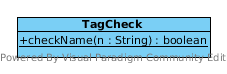
\includegraphics[scale=4, max width=\textwidth, max height=\myheight]{../img/diagrammiClassi/server/validator/TagCheck.png}
				\caption{Diagramma classe - server::validator::TagCheck}
			\end{figure}
		\end{center}\begin{description}
\item[Descrizione] \hfill \\
 Questa classe contiene tutte le funzioni di controllo della validità dei campi del model Tag
\item[Utilizzo] \hfill \\
 Viene utilizzata dai service per effettuare controlli sul model Tag
\item[Metodi] \hfill \\
 \vspace{-7mm}
\begin{itemize}
\item checkName(n : String) : Boolean (Controlla che il nome dell'argomento non sia vuoto)\begin{itemize}
\item n (Il nome dell'argomento da controllare)
\end{itemize}

\end{itemize}

\end{description}

\vspace{0.5cm}
\hypertarget{server::validator::QuestionCheck}{}
\subsubsection[QuestionCheck]{server::validator::QuestionCheck}
\begin{center}
			\begin{figure}[H]
				\centering 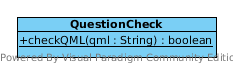
\includegraphics[scale=4, max width=\textwidth, max height=\myheight]{../img/diagrammiClassi/server/validator/QuestionCheck.png}
				\caption{Diagramma classe - server::validator::QuestionCheck}
			\end{figure}
		\end{center}\begin{description}
\item[Descrizione] \hfill \\
 Questa classe contiene tutte le funzioni di controllo della validità dei campi del model Question
\item[Utilizzo] \hfill \\
 Viene utilizzata dai service per effettuare controlli sul model Question
\item[Metodi] \hfill \\
 \vspace{-7mm}
\begin{itemize}
\item checkQML(qml : String) : Boolean (Controlla che la stringa di QML (generalmente quella dell'attributo body del model Question) sia QML valido)\begin{itemize}
\item qml (La stringa in formato QML da controllare)
\end{itemize}

\end{itemize}

\end{description}
